A more general case of a Langevin equation is of the form
\begin{equation}
	\dot{q}=F(q)+\sqrt{Q}\xi(t)\quad\text{with}\quad
	\begin{cases}
		\langle \xi(t)\rangle&=0\\
		\langle \xi(t)\xi(t^\prime)\rangle&=\delta(t-t^\prime)
	\end{cases}
\end{equation}
where the stochastic term represents additive white noise with a zero mean and a Gaussian distribution.\\
The system’s \emph{stationary distribution} is given by the so-called \emph{Fokker-Planck} equation
\begin{equation}{\label{eq:fpe}}
	\dot{p}(q,t)=\frac{\partial}{\partial t}p(q,t)=\underbrace{-\frac{\partial}{\partial q}\{F(q)p(q,t)\}}_{\text{drift}}+\underbrace{\frac{Q}{2}\frac{\partial^2}{\partial q^2}p(q,t)}_{\text{diffusion}}
\end{equation}
\begin{wrapfigure}{r}{0.33\linewidth}
	\centering
	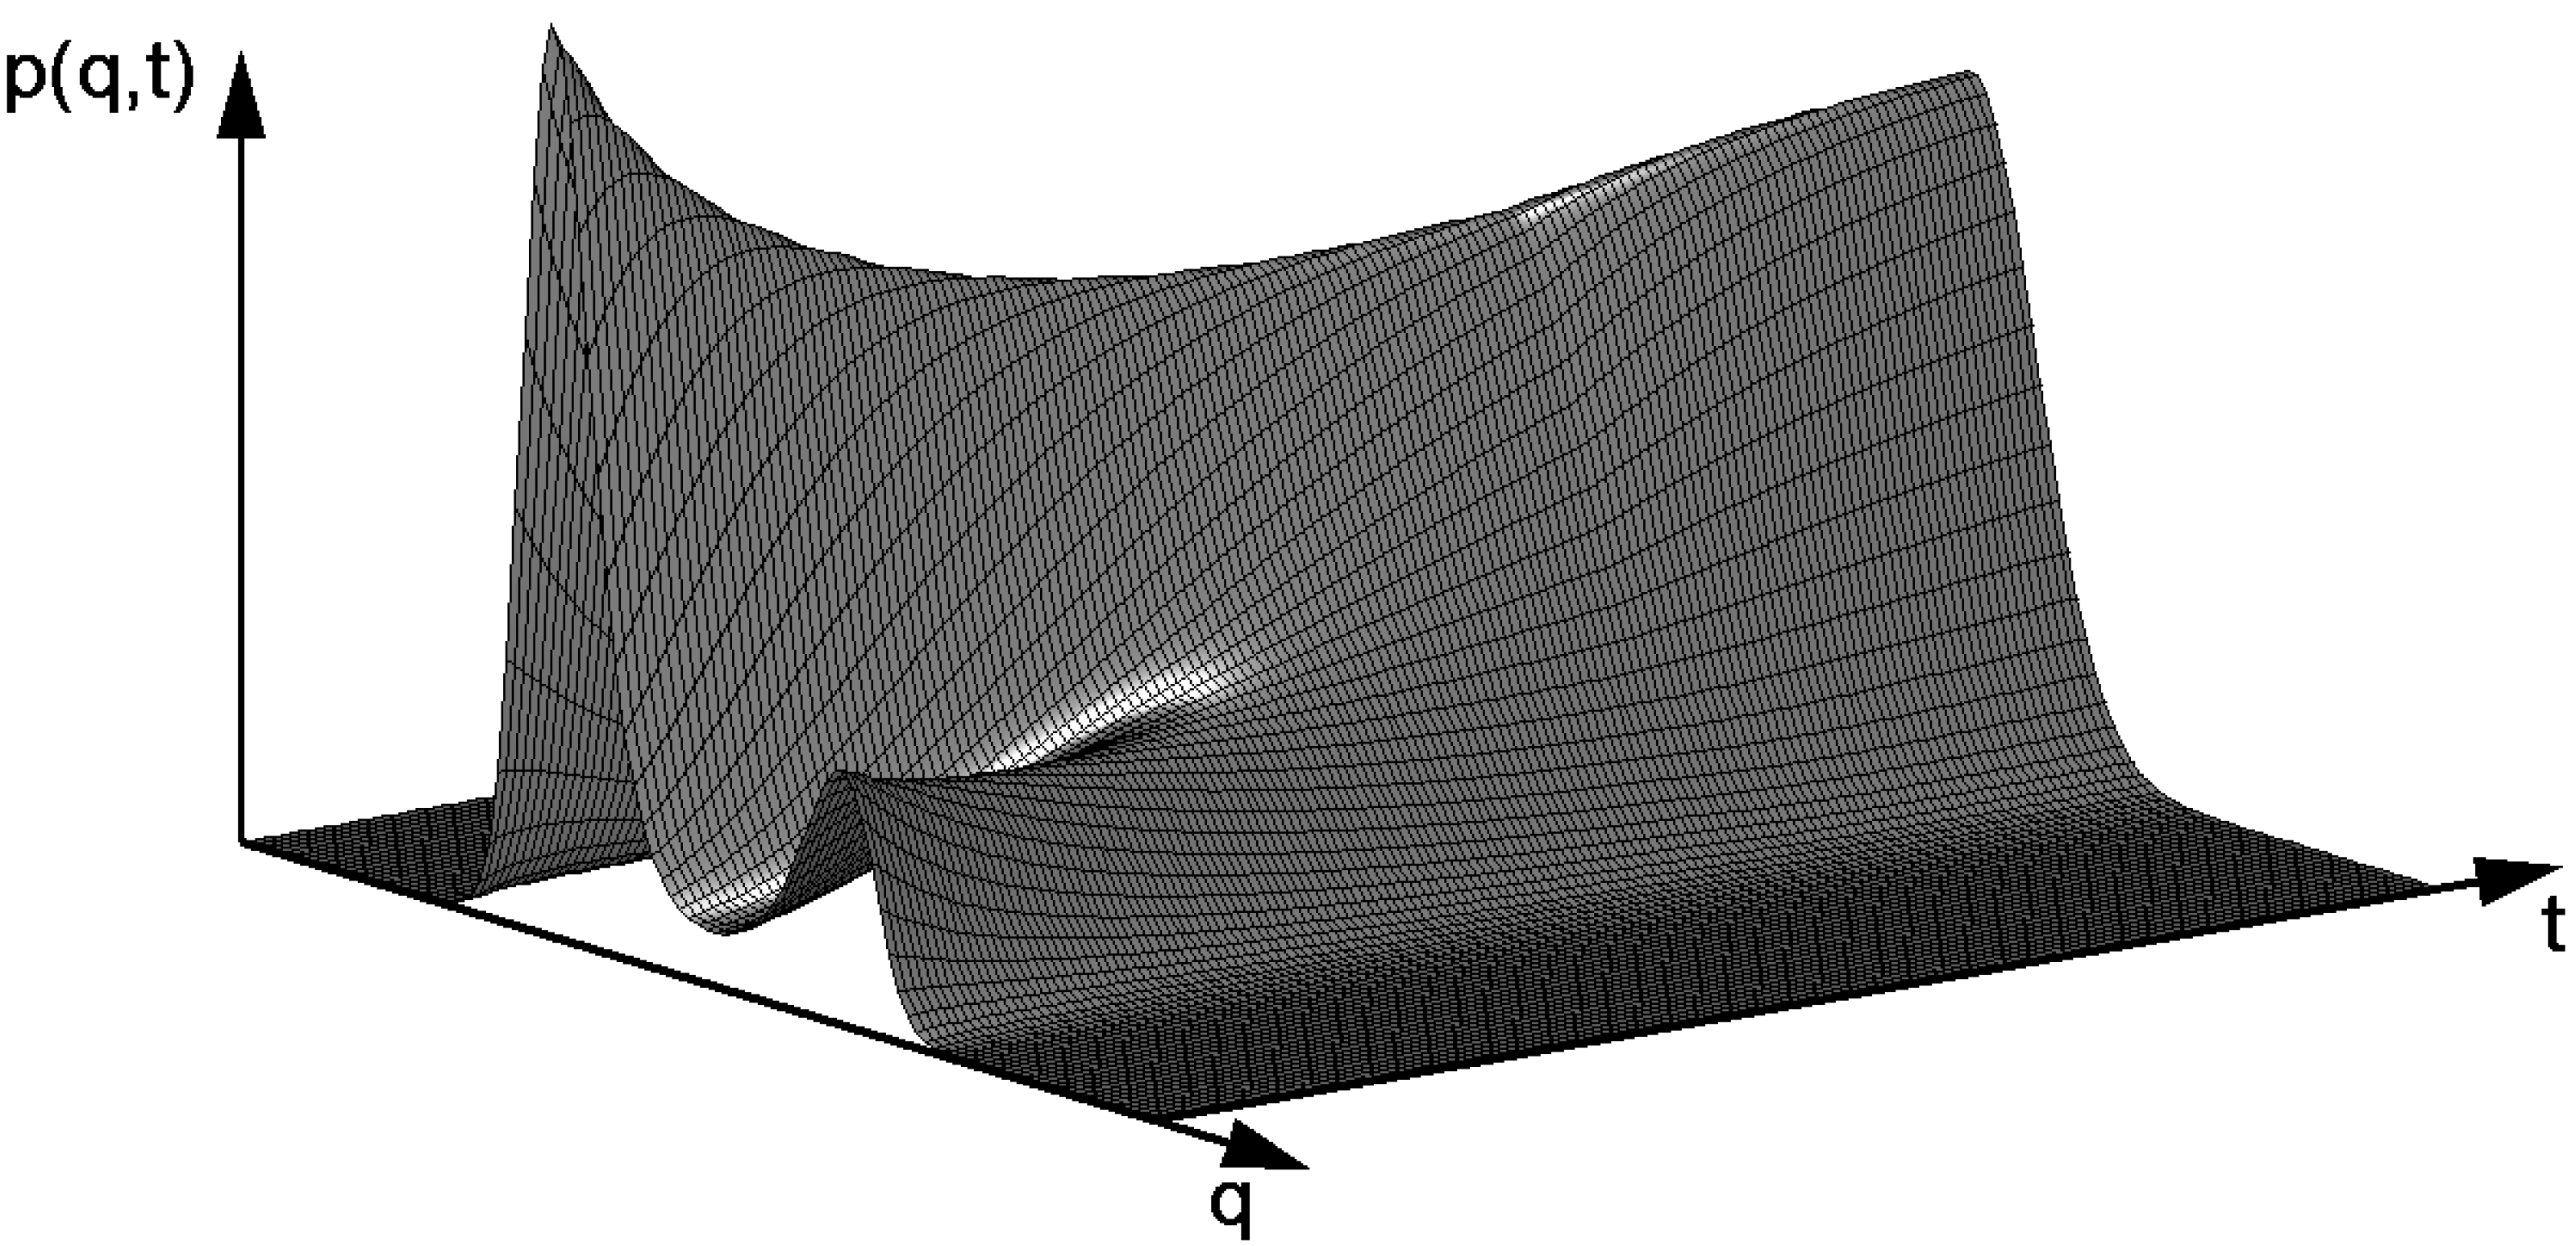
\includegraphics[width=\linewidth]{nsfpe.png}
	\caption{Numerical simulation of a Fokker-Planck equation (\ref{eq:fpe}) where an initial asymmetric distribution with two maxima evolves into a Gaussian.}
	\label{fig:nsfpe}
\end{wrapfigure}
The first term on the right-hand side is called the \emph{drift} term representing the deterministic force in the Langevin equations whereas the second term, the \emph{diffusion} term models the stochastic contributions.
\begin{equation*}
	\begin{aligned}
		\dot{p}(q,t)&=\frac{\partial}{\partial q}\underbrace{\left\{-F(q)p(q,t)+\frac{Q}{2}\frac{\partial}{\partial q}p(q,t)\right\}}_{=\text{constant=0}}=0\quad\rightarrow\quad F(q)p(q)=\frac{Q}{2}\frac{d}{dq}p(q)\\
		p(q)&=e^C e^{\frac{2}{Q}\int F(q)\mathop{dq}}=Ne^{\frac{2}{Q}\int F(q)\mathop{dq}}\quad\text{where}\quad N=\left\{\int_{-\infty}^\infty p(q)\mathop{dq}\right\}^{-1}
	\end{aligned}
\end{equation*}
In Section (\ref{sec:pf}), the potential for dynamical systems was introduced, which can be used now to finally write the stationary distribution in the form
\begin{equation}
	F(q)=-\frac{dV(q)}{dq}\quad\rightarrow\quad p(q)=Ne^{-\frac{2}{Q}V(q)}
\end{equation}